\documentclass[letterpaper, 10 pt, conference]{article}

%\IEEEoverridecommandlockouts
%\overrideIEEEmargins

% The following packages can be found on http:\\www.ctan.org
\usepackage{graphicx} % for pdf, bitmapped graphics files
\usepackage[]{algorithm2e}
\usepackage[noend]{algpseudocode}
%\usepackage{epsfig} % for postscript graphics files
%\usepackage{mathptmx} % assumes new font selection scheme installed
%\usepackage{times} % assumes new font selection scheme installed
\usepackage[margin=1.0in]{geometry}
\usepackage{amsmath} % assumes amsmath package installed
\usepackage{amssymb}  % assumes amsmath package installed
\usepackage{mathtools}
\usepackage{hyperref}

\title{\LARGE \bf
Methods For Solving L0-Norm Minimization Problems In Compressed Sensing
}

\author{Alankar Kotwal (12D070010) and Anand Kalvit (12D070032) \\ Electrical Engineering, IIT Bombay}

\begin{document}
\maketitle
\thispagestyle{empty}
\pagestyle{empty}

\begin{abstract}
Compressed Sensing is a signal processing technique for under-sampling and optimal recovery of a signal, in particular images. It exploits the fact that natural images are sparse in some domain like the Discrete Fourier Transform or Wavelets. The sparsity of the signal can be exploited via optimization to recover it from far fewer samples than required by the Nyquist-Shannon sampling theorem. The sparsity constraint, however, is of a combinatorial nature and is NP-hard. We explore various methods for solving this problem via convex optimization. We plan to use two classes of methods: Orthogonal Matching Pursuit and Rank Minimization to solve this problem.
\end{abstract}

\section{Introduction}
A common goal of signal processing is to reconstruct a signal from a series of sampling measurements. In general, this task is impossible because there is no way to reconstruct a signal during the times that the signal is not measured. Nevertheless, with prior knowledge or assumptions about the signal, it turns out to be possible to perfectly reconstruct a signal from a series of measurements. Over time, engineers have improved their understanding of which assumptions are practical and how they can be generalized.

An early breakthrough in signal processing was the Nyquist-Shannon sampling theorem. It states that if the signal's highest frequency is less than half of the sampling rate, then the signal can be reconstructed perfectly. The main idea is that with prior knowledge about constraints on the signal's frequencies, fewer samples are needed to reconstruct the signal.

Around 2004, Emmanuel Cand\'es, Terence Tao, and David Donoho proved that given knowledge about a signal's sparsity, the signal may be reconstructed with even fewer samples than the sampling theorem requires. This idea is the basis of compressed sensing.

\section{The Compressed Sensing Problem}
Given a signal $\mathbf{x}$, we have its representation in a basis $\mathbf{\Psi}$ given by
$$\mathbf{x} = \mathbf{\Psi \alpha}$$
where $\mathbf{\alpha}$ are the coefficients of $\mathbf{x}$ in the basis represented by the columns of $\mathbf{\Psi}$. $\mathbf{x}$ being sparse in the basis $\mathbf{\Psi}$ means that the cardinality of $\mathbf{\alpha}$ is much less than the number of elements in it. This is the case with natural images and signals in the Fourier, Wavelet or Discrete Cosine Transform domain. 

We consider sampling linear combinations of the components of the signal. This means the sampled version of the signal available to us is 
$$\mathbf{y} = \mathbf{\Phi x}$$
The matrix $\mathbf{\Phi}$ is typically a short and fat matrix, so that the number of columns in $\mathbf{y}$ is much less than the number of elements in $\mathbf{x}$. This gives rise to the `compressive' nature of the measurements. We can reconstruct the signal from less measurements than the number of elements in the signal itself, reducing measurement times and speeding up the acquisition process. In practice the matrix is usually binary, with the result that only some of the elements of $\mathbf{x}$ appear in the elements of $\mathbf{y}$. One has to make sure that the basis $\mathbf{\Psi}$ is `incoherent' with the measurement $\mathbf{\Phi}$, meaning that the measurement vectors (columns of $\mathbf{\Phi}$) are themselves not sparse in the basis $\mathbf{\Psi}$. This is usually done by choosing the matrix $\mathbf{\Phi}$ randomly.

\begin{figure}[thpb]
      \centering
      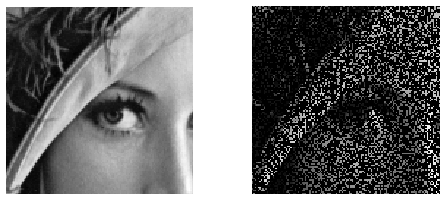
\includegraphics[scale=0.5]{cs-example}
      \caption{An example of compressed sensing in images. Right: The output of the sampling represented as an image. Left: The output from a reconstruction algorithm. Figure taken from https://www.ceremade.dauphine.fr/~peyre/matlab/sparsity/}
      \label{figurelabel}
\end{figure}

\section{Solving Compressed Sensing}

The compressed sensing problem is then to reconstruct $\mathbf{x}$ from $\mathbf{y}$, $\mathbf{\Phi}$ and $\mathbf{\Psi}$. We need to solve for $\mathbf{x}$, given that $$\mathbf{y} = \mathbf{\Phi \Psi \alpha}$$ This is an under-determined linear system. The optimization problem we construct to solve this is
$$\hat{\alpha} = \min_\alpha \|\mathbf{y} - \mathbf{\Phi \Psi \alpha}\|$$
such that $\|\alpha\|_0 \leq K$. The parameter K controls the sparsity of the estimated $\alpha$.

However, this is not a convex program since the L0 norm in the constraint is not convex. We aim to use approximation methods to solve this problem.

\subsection{Matching Pursuit}
Matching pursuit \cite{wiki_mp} is a type of sparse approximation which involves finding the ``best matching" projections of multidimensional data onto a dictionary $\mathcal{D}$. The basic idea is to represent the signal $\mathcal{Y}(x)$ as a weighted sum of functions $f_{n}(x)$ (called atoms) taken from $\mathcal{D}$:
$$\mathcal{Y}(x) = \sum_{n=0}^{N} a_n f_{n}(x)$$
In our setting the dictionary is the basis in which our signal is sparse in (like DCT or Fourier coefficients, the matrix $\mathbf{\Phi \Psi}$). We restrict the number of coefficients to $N$ to enforce sparsity. Matching pursuit provides a way to find the `best' representative atoms so that the signal is represented faithfully while honouring the sparsity constraint.

\begin{algorithm}[]
 \KwData{Signal: $\mathcal{Y}(x)$, dictionary $\mathcal{D}$}
 \KwResult{List of coefficients: $\left(a_n, f_{n}(x)\right)$.}
 Initialization\: \\
 $R_1(x)\,\leftarrow\,\mathcal{Y}(x)$ \\
 $n\,\leftarrow\,1;$\\
 \While{$\|R_n(x)\| < \mathrm{threshold}$}{
   $f_{n}(x) \leftarrow \text{arg} \max_{f_i(x) \in \mathcal{D}} \|R_n(x) - f_i(x)\|$ \\
   $a_n \leftarrow \|R_n(x) - f_i(x)\|\;$ \\
   $R_{n+1}(x) \leftarrow R_n(x) - a_n f_n(x)$ \\
   $n \leftarrow n+1$
   
 }
 \caption{Matching Pursuit}
\end{algorithm}

As seen in Algorithm 1, the algorithm picks the dictionary element that is the most coherent with the residual function at a given iteration. This tries to ensure that we pick the least number of elements from the dictionary, thus accounting for the sparsity of the signal. A major drawback of this algorithm is that if the dictionary atoms are not orthogonal, it can pick the same atom twice. The modification that corrects this is called Orthogonal Matching Pursuit.

\subsection{Orthogonal Matching Pursuit}
Orthogonal Matching Pursuit solves the above problem by building a `support set' of atoms, that is, a set of atoms that have already been used in the reconstruction of the signal. The algorithm goes as shown in Algorithm 2.

\begin{algorithm}[]
 \KwData{Signal: $\mathcal{Y}(x)$, dictionary $\mathcal{D}$}
 \KwResult{List of coefficients: $\left(a_n, f_{n}(x)\right)$.}
 Initialization\: \\
 $R_1(x)\,\leftarrow\,\mathcal{Y}(x)$ \\
 $n\,\leftarrow\,1;$\\
 $\mathcal{S} \leftarrow \Phi$ \\
 \While{$\|R_n(x)\| < \mathrm{threshold}$}{
   $f_{n}(x) \leftarrow \text{arg} \max_{f_i(x) \in \mathcal{D}} \|R_n(x) - f_i(x)\|$
   $\mathcal{S} = \mathcal{S} \cup f_n(x)$ \\
   $\mathbf{a} \leftarrow \text{arg} \min_{w \in \mathbb{R}^k} \|\mathcal{Y}(x) - \sum_{f_i(x) \in \mathcal{S}} w_i f_i(x)\|\;$ \\
   $R_{n+1}(x) \leftarrow \mathcal{Y}(x) - \sum a_n f_n(x)$ \\
   $n \leftarrow n+1$
 }
 \caption{Orthogonal Matching Pursuit}
\end{algorithm}

Since the residual calculation in the algorithm makes sure that the residual at each step is orthogonal to all the atoms in the support set, no atom can be picked twice by OMP. This makes OMP a good choice for low-computation sparse signal recovery.

\subsection{Difference-of-Convex Functions Approximation}
This approach involves relieving the non-convexity of the constraint by constructing a convex series of approximations to it. This convex series of constraints approaches the non-convex L0 norm constraint as a parameter approaches zero.

Given the L0 norm constraint
$\|x\|_0 = \sum sgn(|x_i|)$
we construct the following underestimate for $sgn(|z|)$:
\begin{equation*}
\begin{aligned}
\psi(x, t) &= min{\left(1, \frac{|x|}{t}\right)} \\
		   &= \frac{|x|}{t} - \frac{(x-t)^{+} + (-x-t)^{+}}{t} \\
		   &= \frac{h(x, 0)}{t} - \frac{h(x, t)}{t}
\end{aligned}
\end{equation*}
where $z^{+} = max(z, 0)$ and $h(x, t) = (x-t)^{+} + (-x-t)^{+}$. $h(x, t)$ is a convex function of $x$, hence this is a difference-of-convex functions. Summing over all components of the representation of the signal, we have
\begin{equation*}
\begin{aligned}
\phi(x, t) &= \sum \psi(x_i, t) \\
		   &= \frac{\|x\|_1}{t} - \frac{g(x, t)}{t}
\end{aligned}
\end{equation*}
where $g(x, t) = \sum h(x_i, t)$. Next, we construct a convex underestimate for this by linearizing the negative convex function by constructing its affine approximation around the current estimate. Consider a $\xi \in \partial g(x, t)$. We have, at a given $y$
$$\phi(x, t) \leq u(x, y, \xi, t) \coloneqq \frac{\|x\|_1}{t} - \frac{1}{t}\left[g(y, t) - \xi^T (x-y)\right]$$
Using this the compressed sensing problem can be cast into the following series of optimization problems indexed by $t$:
$$(P_t(y, \xi)) \hspace{20pt} \min \|\mathbf{y} - \mathbf{\Phi \Psi x}\|$$
such that
$$\frac{\|x\|_1}{t} - \frac{1}{t}\left[g(y, t) - \xi^T (x-y)\right] \leq K$$
We can get rid of the non-smooth L1 norm by casting the problem as:
$$(CP_t(y, \xi)) \hspace{20pt} \min \|\mathbf{y} - \mathbf{\Phi \Psi x}\|$$
such that
$$\frac{z}{t} - \frac{1}{t}\left[g(y, t) - \xi^T (x-y)\right] \leq K$$
$$-x_i \leq z_i \leq x_i$$
It can be proved that as $t \rightarrow 0$, the solution to this series of convex programs converges to the solution to the L0 norm optimization problem (see the analysis section).

\begin{algorithm}[]
 \KwData{Signal: $\mathcal{Y}(x)$, dictionary $\mathcal{D} \equiv \mathbf{\Phi \Psi}, \epsilon > 0$}
 \KwResult{$\alpha$}
 Initialization\: \\
 $t \leftarrow t_0 > 0$ \\
 $x \leftarrow x^0\text{ as starting guess}$ \\
 $\xi^0 \in \partial g(x^0, t)$ \\
 $k \leftarrow 0$ \\
 \While{$\|x^{k} - x^{k-1}\| > \epsilon$}{
   Solve $(CP_t(x^k, \xi^k))$, set solution to $x^{k+1}, z^{k+1}$
   $k \leftarrow k+1$
 }
 \caption{SCA Method}
\end{algorithm}

The entire algorithm can then be written as shown in Algorithm 3.
The problem $(CP_t(x^k, \xi^k))$ can be solved using KKT conditions.

\subsection{Penalty Decomposition Method}
General rank minimization problems with rank appearing
in either objective function or constraint can be solved as lower dimensional vector optimization problems \cite{pd}. As a consequence, we establish that a class of rank minimization problems have closed form solutions. Using this result, we then propose penalty decomposition methods for general rank minimization problems. Penalty Decomposition methods work by formulating a penalty function, minimizing which amounts to minimizing our objective function.
\\ \\
\newpage
\noindent The Compressed Sensing problem can be reformulated as:
$$min_{(X,Y)}\left\{{f(X) : X-Y=0\,,\, X \in \mathcal{X}\,,\, Y \in \mathcal{Y}}\right\}$$
where $f(X)$ is the C.S objective function and Y is defined as:
$$Y:=\left\{{Y \in \mathcal{Y}\,  |\,  rank(Y) \le r}\right\}$$
Given a penalty parameter $\rho$ $\ge$ 0, the associated quadratic penalty function for the above C.S. problem is defined as:
$$Q_{\rho} := {f(X)+\frac{\rho}{2} {{\|X-Y \|}_F}^2}$$
We use \emph{Block Coordinate Descent} to minimize the above penalty function. Using results from \cite{pd}, the minimizer $X$ is related to the minimizer $x$ of the following vector optimization problem as $X=UD(x){V}^T$ where $D(x)$ is a diagonal matrix with elements of $x$ as the diagonal entries and $U\Sigma V^T$ is the \emph{Singular Value Decomposition} of $Y$.
$$Q_{\rho} := {f(x)+\frac{\rho}{2} {{\|x-y \|}_2}^2}$$
where $$y:=\left\{{y \in \mathcal{Y}\, |\, {\|y\|}_0 \le r}\right\}$$
\\ \\
The L0 norm minimization problem thus becomes tractable under certain conditions (which are discussed in the \emph{Analysis} section later) using this methodology.

\section{Results}
We test out the compressed sensing problem as solved by all three methods on the standard Barbara image. The image at two resolutions is shown below: \\ \\
\centerline{
\includegraphics[scale=2.6]{barbara} 
\includegraphics[scale=0.5]{barbara256}} \\ \\ 
We extract 8 $\times$ 8 patches from the image and apply compressed sensing on them. We extract compressed measurements from patches by multiplying the vectorized patch with a fixed random $64 \times 64f$ matrix where $f$ is the level of compression we achieve. We thus aim to reconstruct the entire patch from measurements that are less in number by a factor of $f$. We then add the reconstructed patches back to form the output image. Results are shown in the subsequent subsections.

\newpage
\subsection{Orthogonal Matching Pursuit}
OMP results for $f=0.1$, $f=0.2$ and $f=0.6$ respectively, on the reduced image: \\ \\
\centerline{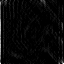
\includegraphics[scale=2]{out-omp-10p} 
\includegraphics[scale=2.6]{out-omp-20p}} \\ \\
\centerline{ 
\includegraphics[scale=2.6]{out-omp-60p}} \\ \\
Clearly, the level of reconstructed detail increases as we increase the number of measurements, as expected. 

\noindent OMP results for $f=0.1$, $f=0.2$ and $f=0.6$ respectively, on the full resolution image: \\ \\
\centerline{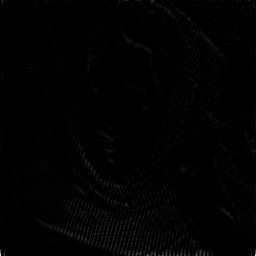
\includegraphics[scale=0.5]{out-omp4x-10p} 
\includegraphics[scale=0.5]{out-omp4x-20p}} \\ \\
\centerline{ 
\includegraphics[scale=0.5]{out-omp4x-60p}} \\ \\


\subsection{Difference-of-Convex Functions Approximation}
SCA results for $f=0.1$, $f=0.2$ and $f=0.6$ respectively, on the reduced image: \\ \\
\centerline{
\includegraphics[scale=2.3]{out-sca-10p} 
\includegraphics[scale=2.3]{out-sca-20p}} \\ \\
\centerline{ 
\includegraphics[scale=2.3]{out-sca-60p}} \\ \\
Clearly, the level of reconstructed detail increases as we increase the number of measurements, as expected. It is interesting to note that \textbf{all} of the pixels in the $f=0.2$ output are within $\pm 15$ units of the ground truth. The mean absolute error is around 1.8, which on a scale of 255 is $0.72\%$. On the contrary, the corresponding figure for the OMP output is 10, which is more than 6 times our error.

\noindent SCA results for $f=0.1$, $f=0.2$ and $f=0.6$ respectively, on the full resolution image: \\ \\
\centerline{
\includegraphics[scale=0.5]{out-sca4x-10p} 
\includegraphics[scale=0.5]{out-sca4x-20p}} \\ \\
\centerline{ 
\includegraphics[scale=0.5]{out-sca4x-60p}} \\ \\

\noindent As we see here, SCA can recover as much detail with a fraction $f=0.2$ of measurements as OMP can at $f=0.6$. In fact, in the full resolution case, we see that SCA recovers the original image almost \textbf{exactly} in the $f=0.2$ case. This is considerable savings on exposure time, about a factor of 5 over traditional imaging, and a factor of 3 over OMP.

\subsection{Penalty Decomposition Method}

We deal only with the full resolution image here, but with different sparsity constraints on the reconstructed image. The value of epsilon for the inner loop termination criterion has been set to 0.05 (5$\%$) and that for the outer loop to 15 ($5.8\%$ of 256). For the perturbation check to ensure that a stationary point corresponds to a minimum and not a saddle, the ratio-factor $\frac{q_{\rho_k}(\tilde{x}^k,\tilde{y}^k)}{q_{\rho_k}(x^k,y^k)}$ has been set to 0.5.\\ \\
PD results for $f=0.1$, $f=0.2$ and $f=0.6$ respectively, with 20$\%$ sparsity constraint on the reconstructed image: \\ \\
\centerline{
\includegraphics[scale=0.5]{out-PD-0_1f-0_2s-full-pc.png} 
\includegraphics[scale=0.5]{out-PD-0_2f-0_2s-full-pc.png}} \\ \\
\centerline{ 
\includegraphics[scale=0.5]{out-PD-0_6f-0_2s-full-pc.png}} \\ \\
Clearly, the level of reconstructed detail increases as we increase the number of measurements, as expected. An interesting fact is, even though OMP seems to have performed slightly better for $f=0.2$ and $f=0.6$, the run-times for the 2 algorithms are drastically different. The PD method achieves this level of reconstruction detail in a fraction of OMP's run-time. What this means is, we can afford to make our loop termination and perturbation check criteria much stricter, to get near-perfect reconstructions. 
\\ \\
\newpage
\noindent PD results for $f=0.1$, $f=0.2$ and $f=0.6$ respectively, with 30$\%$ sparsity constraint on the reconstructed image: \\ \\
\centerline{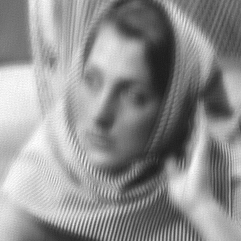
\includegraphics[scale=0.5]{out-PD-0_1f-0_3s-full-pc.png} 
\includegraphics[scale=0.5]{out-PD-0_2f-0_3s-full-pc.png}} \\ \\
\centerline{ 
\includegraphics[scale=0.5]{out-PD-0_6f-0_3s-full-pc.png}} \\ \\

\noindent Clearly, the results become better with less stricter constraints on the sparsity of the reconstructed image. We can still have finer reconstructions by  making the termination criteria stricter and having a more robust perturbation check, but at the expense of run-time. However, the merit of this method lies in the fact that, for a specified level of reconstruction precision, the PD algorithm performs the fastest among the 3.

\section{Analysis}
Now that we showed empirically that the methods work, we present proofs that under certain conditions, the problem under consideration is actually solved exactly by our algorithms.

\subsection{Difference-of-Convex Functions Approximation}
Consider the generic problem given by $$\hat{\alpha} = \min_\alpha \|\mathbf{y} - \mathbf{A \alpha}\| < \epsilon$$
such that $\|\alpha\|_0 \leq K$. We constructed an underestimate for the L0 norm of $\alpha$ parameterized by t, given by $\phi(\alpha, t)$. We have, $\|\alpha\|_0, \phi(\alpha, t) \geq 0$. 

Now consider the feasible sets of the two problems. Let $F_0$ be the feasible set of the original problem and $F_t$ be the feasible set of problem $P_t$. Thus,
$$F_0 = \{ \alpha \in \mathbb{R}^n \ :\ \|\alpha\|_0 \leq K \} \text{ and } F_t = \{ \alpha \in \mathbb{R}^n \ :\ \phi(\alpha, t) \leq K \}$$
It is easy to see that both of these are closed sets in $\mathbb{R}$. Therefore, since $\|\alpha\|_0 \geq \phi(\alpha, t)$, we have, $$F_0 \subseteq F_t \text{ for all } t>0$$

Now, we know, $\phi(\alpha, t_2) \leq \phi(\alpha, t_1)$ for any $0 < t_1 \leq t_2$. Therefore, $F_0 \subset F_{t_1} \subseteq F_{t_2}$ for any $0 < t_1 \leq t_2$. Given this we know that $\lim_{t \rightarrow 0^+} F_t$ exists and $F_0 \subset \lim_{t \rightarrow 0^+} F_t$. Next, by the definition of $\psi(z, t)$ as the underestimate for $|sgn(z)|$, we know $\lim_{t \rightarrow 0} \psi(z, t) = |sgn(z)|$. This gives, by summation over components of $\alpha$, $\lim_{t \rightarrow 0} \phi(\alpha, t) = \|\alpha\|_0$. This, therefore, means $\lim_{t \rightarrow 0} F_t = F_0$ because of the inclusion property proved above. Now, the objective function, being an L2 norm of a linear function of the optimizing variable, is convex. Thus, the problem $P_1$ with a feasible set that is the superset of another problem $P_2$ with the same objective function can potentially achieve a lower optimal value than $P_2$. Thus, if $v(P)$ denotes the optimal value of the problem $P$, we have $v(P_t) \leq v(P_0)$. Now, since we proved that the constraint of $P_t$ converges to the constraint of $P_0$ as $t \rightarrow 0$, we have $\lim_{t \rightarrow 0} v(P_t) = v(P)$.

Next, the $u(\alpha, \alpha_0, \xi, t)$ was constructed for the DC function $\phi(\alpha, t)$ around the point $\alpha_0$, with $\phi(\alpha, t) \leq u(\alpha, \alpha_0, \xi, t)$. Following the same logic as above, the feasible sets of $CP_t$, given by $$F_t(\alpha_0, \xi) = \{ \alpha \in \mathbb{R}^n \ :\ u(\alpha, \alpha_0, \xi, t) \leq K \}$$ follow $F_t(\alpha_0, \xi) \subseteq F_t \text{ for all } t > 0,\  \xi \in \partial\phi(\alpha_0, t)$. This means, $v(P_t(\alpha_0, \xi)) \geq v(P_t)\text{ for all } t > 0,\  \xi \in \partial\phi(\alpha_0, t)$.

We further relax the non-smoothness of the constraint in $P_t(\alpha_0, \xi)$ by introducing additional variables $z_i$, to form the problem $CP_t(\alpha_0, \xi)$. This step does not change the problem and forces $z_i = |\alpha_i|$. The constraint introduced, $-z_i \leq \alpha_i \leq z_i$ is equivalent to saying $|\alpha_i| \leq z_i$. The feasible sets over x for $CP_t(\alpha_0, \xi)$, are, then, smaller subsets of the feasible sets over x for $P_t(\alpha_0, \xi)$ for any $|x_i| < z_i$ (since the objective function is a non-decreasing function as $\alpha_i$ moves away from the optimum). Hence, the minimum always lies in the difference of the feasible sets for $P_t(\alpha_0, \xi)$ and $CP_t(\alpha_0, \xi)$, except when $|x_i| = z_i$, when both minima are equal. Thus, if there exists a solution to $P_t(\alpha_0, \xi)$, given by $x^*$, there is a solution to $CP_t(\alpha_0, \xi)$, given by $x^*, z^*$ where $z_i = |x_i|$. Thus $P_t(\alpha_0, \xi)$ and $P_t(\alpha_0, \xi)$ are equivalent optimization problems. We use the fact that $CP_t(\alpha_0, \xi)$ is smooth to derive a condition on the optimum for $CP_t(\alpha_0, \xi)$, and therefore the optimum of $P_t(\alpha_0, \xi)$.

Now that we have shown the relation between $P$ and $P_t$, we will analyse the optimum of $P_t$. Let $\alpha^*$ be a local optimum for $P_t$. The KKT conditions (formulated with respect to the sub-gradient) imply that there exists a non-negative $\mu^*$ such that
$$0 \in 2A^TA\alpha^* + A^Ty + \mu^* \partial \phi(\alpha^*, t),$$
$$\mu^* (\phi(\alpha^*, t) - K) = 0$$
A point $\alpha^*$ satisfying these is called a KKT point for the problem $P_t$. 

The corresponding conditions for the problem $CP_t(\alpha_0, \xi)$ can be written, with $(\tilde{\alpha}, \tilde{z})$ solving $CP_t(\alpha_0, \xi)$, there exist non-negative multipliers $\tilde{\zeta}, \tilde{\beta}, \tilde{\mu}$ such that
$$2A^TA\tilde{\alpha} + A^Ty + \tilde{\zeta} - \tilde{\beta} - \frac{1}{t}\tilde{\mu}\xi = 0,$$
$$\frac{1}{t}\tilde{\mu}e - \tilde{\zeta} - \tilde{\beta} = 0,$$
$$\tilde{\mu} \left( \frac{1}{t} e^T \tilde{z} - \frac{1}{t} g(\alpha_0, t) - K \right) = 0,$$
$$\tilde{\zeta_i} (z_i - \tilde{\alpha}_i) = 0,$$
$$\tilde{\beta_i} (z_i + \tilde{\alpha}_i) = 0$$

\noindent We already showed that $\tilde{\alpha_i} = \tilde{z_i}$. This implies, $\tilde{\alpha_i} > 0 \implies \tilde{\beta_i} = 0$ and $\tilde{\alpha_i} < 0 \implies \tilde{\zeta_i} = 0$. Thus, $\tilde{\zeta_i} = (1/t)\tilde{\mu}$ when $\tilde{\alpha_i} > 0$ and $\tilde{\beta_i} = (1/t)\tilde{\mu}$ when $\tilde{\alpha_i} < 0$. When $\tilde{\alpha_i} = 0$, $\tilde{\zeta} - \tilde{\beta} \in \left[-(1/t)\tilde{\mu}, (1/t)\tilde{\mu}\right]$. This implies that $\tilde{\zeta} - \tilde{\beta} - (1/t) \tilde{\mu} \xi \in \tilde{\mu} \partial\phi(\tilde{\alpha_i}, t)$. Then, the first equation in the $CP_t(\alpha_0, \xi)$ KKT conditions implies the first equation in the $P_t$ KKT conditions, and the constraint conditions in $CP_t(\alpha_0, \xi)$ give the constraint conditions in $P_t$, if $\tilde{\alpha} = \alpha_0$. Thus, we prove that if there exists a solution $(\alpha_0, |\alpha_0|)$ to $CP_t(\alpha_0, \xi)$ for some $\xi \in g(\alpha_0, t)$, that is the solution for $P_t$.

With this, we can generate a series of subproblems by solving $CP_t(\alpha^k, \xi^k)$, and setting the solution to $\alpha^{k+1}$. If the difference $\alpha^{k+1} - \alpha^{k}$ is small (in terms of some norm), we can say that $\alpha^{k}$ approximately solves $CP_t(\alpha^k, \xi^k)$. By the above proof, we have that $\alpha^k$ is a KKT point for $P_t$. As we proved at the beginning of the section, the problem $P_t$ converges to the original compressed sensing problem $P$ as $t \rightarrow 0$. This means, choosing a small t we almost exactly solve the compressed sensing problem with our successive convex approximations.

\subsection{Penalty Decomposition Method}

The Compressive Sensing problem we are addressing, can be formulated as :-
$$min_{x\in{\mathbb{R}^{\textit{p}}}}\ \left\lbrace\frac{1}{2} {\|Ax-b \|}_{2}^{2}\right\rbrace$$
such that
$$\|x\|_0\leq r$$
where $A\in \mathbb{R}^{n \times p}$ is a data matrix which is short and fat i.e. ($n<p$), $B\in \mathbb{R}^n$ is an observation vector, and $r\in [1, p]$ is some integer for controlling the sparsity of the solution. The traditional approach to solve the above problem is to solve the $l1$-norm regularization, namely,
$$min_{x\in{\mathbb{R}^{\textit{p}}}}\ \left\lbrace\frac{1}{2} {\|Ax-b \|}_{2}^{2}\ +\ \lambda\|x\|_1\right\rbrace$$
where $\lambda\geq 0$ is a regularization parameter. We, in this paper, attempt to solve the original problem directly using the PD method.
\\
For ease of representation, we denote the objective function by $f(x)$ and pose the problem as :
\begin{equation}
min_{x}\ \left\lbrace{f(x)\ :\ \|x\|_0\leq r,\ x\in{\textit{X}}}\right\rbrace 
\end{equation}
We first reformulate the above problem as an equivalent rank minimization problem and then apply the PD method proposed in \cite{pd} to solve the latter problem. By utilizing the special structures of the problem, we then transform all matrix operations of the PD method to vector operations and obtain a PD method that only involves vector operations.
\\ \\
We now define the set $\textit{X}_M$ and the function $\textit{f}_M$ as follows :
$$\chi_M = \left\lbrace{{D(x):x\in{\chi}}}\right\rbrace,\ \ \ \ \ \ \ \textit{f}_M(X)=\textit{f}\ ({\textit{D}}^{\ast}(X))\ \ \forall\ X\in{D^n}$$ 
where $D(x)$ is a diagonal matrix constructed with the elements of $x$, $D^n$ represents the space of all $n$x$n$ diagonal matrices, $D^{\ast}(X)\in{\mathbb{R}^n}$ is the vector extracted from the diagonal of X. Then, the matrix equivalent formulation of (1) can be written as :
\begin{equation}
min_{X}\ \left\lbrace{f_M(X)\ :\ rank(X)\leq r,\ X\in{{\chi}_M}}\right\rbrace 
\end{equation}
\\
We define the space of all nxn real symmetric matrices, with rank less than or equal to r as :
$$\gamma_M := \left\lbrace{Y\in{S^n}\ |\ rank(Y)\leq{r}}\right\rbrace$$
We now add a quadratic penalty function to our objective function to get the new objective as :
$$Q_{\rho}(X,Y):=f_M(X)+\frac{\rho}{2}\|X-Y\|_{F}^{2}$$
Since we know from the Matrix Algebra that every real symmetric matrix is orthonormally diagonalizable, we write the singular value decomposition of $Y$ as :
$$Y=UDU^{T}$$
where $U\in{R^{n \times r}}$, $D\in{D^r}$. We now present a PD method to solve (2).
\newpage
\subsubsection{The Algorithm}

Let $\left\lbrace\epsilon_k\right\rbrace$ be a positive decreasing sequence. Let ̺$\rho > 0$, $\sigma > 1$ be given. Choose an arbitrary $Y_0^0\in{\gamma_M}$ and a constant $\Gamma\geq max\left\lbrace{f(x^{feas}),\ min_{X\in{\chi_M}}\ Q_{\rho_0}(X,Y_0^0)}\right\rbrace$. Set $k=0$.
\begin{enumerate}
\item Set $l=0$ and apply the block coordinate descent (BCD) method \cite{BCD} to find an approximate solution $(X_k,Y_k)\in \chi_M \times \gamma_M$ for the penalty subproblem
$$ min\ \left\lbrace{Q_{\rho_k}(X,Y)\ :\ X\in\chi_M,\ Y\in{{\gamma}_M}}\right\rbrace $$
by performing steps (a) - (d).
\begin{enumerate}
\item Solve $ X_{l+1}^k \in\ Arg\ min_{\bf X\in{\chi_M}}\ Q_{\rho_k}(X,Y_l^k)$.
\item Solve $ Y_{l+1}^k \in\ Arg\ min_{\bf Y\in{\gamma_M}}\ Q_{\rho_k}(X_{l+1}^k,Y)$.
\item Set $(X^k,Y^k):=(X^{l+1},Y^{l+1})$. Then, if $(X^k,Y^k)$ satisfies the following conditions :
\begin{itemize}
\item distance $(-\nabla_{X}Q_{\rho_k}(X^k,Y^k),\ N_{{\chi}_M}(X^k))\leq{\epsilon_k}$, \\
where $N_{{\chi}_M}(X^k)$ is the normal to the cone of $\chi_M$ at $X^k$.
\item $\|\nabla_{U}Q_{\rho_k}(X^k,U^kD^k(U^k)^T)\|_F\leq\epsilon_k$,
\item $\|\nabla_{D}Q_{\rho_k}(X^k,U^kD^k(U^k)^T)\|_F\leq\epsilon_k$,
\end{itemize}
then, go to step (2).
\item Set $l\leftarrow l+1$ and go to step (a).
\end{enumerate}

\item Set $\rho_{k+1}:=\sigma\rho_k.$
\item If $min_{X\in\chi_M}\ Q_{\rho_{k+1}}(X,Y^K)>\Gamma$, set $Y_0^{k+1}:=D(x^{feas})$. Otherwise, set $Y_0^{k+1}:=Y^k$.
\item Set $k\leftarrow k+1$ and go to step (1).
\end{enumerate}

\subsubsection{Analysis}

The conditions listed under step 1(c) are basically the first order optimality (i.e., KKT) conditions of (2). Elaborate proof can be found in \cite{PDlong}. Intuitively, the first condition can be seen as a reformulation of the condition of alignment of normals of the constraint and the objective functions at a critical point of the Lagrangian. $Y$ is parametrized in terms of $U$ and $D$. The second and third conditions are for the change in $Q_{\rho_k}(X,Y)$ along any $D$ or $U$ at $(X^k,Y^k)$ being 0. These 3 are the conditions for any $(X^k,Y^k)$ to be a critical point of 
$Q_{\rho_k}(X,Y)$.
\\ \\
By using the special structures of the matrices involved, the above PD method can be transformed into one that only involves vector operations. Before proceeding, we state the following equivalents :

$$\gamma := \left\lbrace{y\in{\mathbb{R}^n}:\|y\|_0 \leq{r}}\right\rbrace$$
$$q_{\rho}(x,y):=f(x)+\frac{\rho}{2}\|x-y\|_{2}^{2}$$
$$X_{l+1}^k=D(x_{l+1}^k)$$
$$Y_{l+1}^k=D(y_{l+1}^k)$$
where $D$ is the diagonalization operator. We now present the PD method for solving (1).
\\ \\
Let ̺$\rho > 0$, $\sigma > 1$ be given. Choose an arbitrary $y_0^0\in{\gamma}$ and a constant $\Gamma\geq max\left\lbrace{f(x^{feas}),\ min_{x\in{\chi}}\ q_{\rho_0}(x,y_0^0)}\right\rbrace$. Set $k=0$.
\begin{enumerate}
\item Set $l=0$ and apply the block coordinate descent (BCD) method to find an approximate solution $(x_k,y_k)\in \chi \times \gamma$ for the penalty subproblem
\begin{equation}
min\ \left\lbrace{q_{\rho_k}(x,y)\ :\ x\in\chi,\ y\in{{\gamma}}}\right\rbrace 
\end{equation}
by performing steps (a) - (d).
\begin{enumerate}
\item Solve $ x_{l+1}^k \in\ Arg\ min_{\bf x\in{\chi}}\ q_{\rho_k}(x,y_l^k)$. For our choice of $f(x)$, this is a standard quadratic program over a convex domain $\chi$. Hence, a closed form solution exists. 
\item Solve $ y_{l+1}^k \in\ Arg\ min_{\bf y\in{\gamma}}\ q_{\rho_k}(x_{l+1}^k,y)$. $\gamma$ is not a convex domain. $y^k_{l+1}$ is obtained as the best r-sparse approximation to $x^k_{l+1}$.
\item Set $(x^k,y^k):=(x^{l+1},y^{l+1})$. Check the inner stopping criteria. If satisfied, go to step 2.
\item Set $l\leftarrow l+1$ and go to step (a).
\end{enumerate}

\item Set $\rho_{k+1}:=\sigma\rho_k.$
\item If $min_{x\in\chi}\ q_{\rho_{k+1}}(x,y^k)>\Gamma$, set $y_0^{k+1}:=x^{feas}$. Otherwise, set $y_0^{k+1}:=y^k$.
\item Set $k\leftarrow k+1$ and go to step (1).
\end{enumerate}
\ \\
Practically, it is hard to analytically verify the inner  stopping criteria unless $\chi$ is simple. However, on the other hand, we observe that the sequence $\left\lbrace{q_{\rho_k}(x_l^k,y_l^k)}\right\rbrace$ is non-increasing for any fixed $k$. In practical implementation, it is thus reasonable to terminate the BCD method based on the progress of $\left\lbrace{q_{\rho_k}(x_l^k,y_l^k)}\right\rbrace$. Thus, a reasonable termination criterion for the BCD method is :
$$max\left\lbrace{\frac{\|x_l^k-x_{l-1}^k\|_{\infty}}{max(\|x_l^k\|_{\infty},1)},\frac{\|y_l^k-y_{l-1}^k\|_{\infty}}{max(\|y_l^k\|_{\infty},1)}}\right\rbrace \leq \epsilon_0$$
for some $\epsilon_0>0$. Similarly, we can terminate the outer iterations of the above method once ${\|x^k-y^k\|}_{\infty} \leq {\epsilon}_{1}$, for some $\epsilon_1>0$.

\subsubsection{Convergence}

Given that problem (3) is non-convex, the BCD method may converge to a stationary point. To enhance the quality of approximate solutions, one may execute the BCD method
multiple times starting from a suitable perturbation of the current approximate solution. In detail, at the $k^{th}$ outer iteration, let $(x_k,y_k)$ be a current approximate solution of (3) obtained by the BCD
method, and let $r_k=\|y^k\|_0$. Assume that $r_k > 1$. Before starting the $(k + 1)^{th}$ outer iteration, one can apply the BCD method again starting from $y_0^k\in\ Arg\ min\left\lbrace{\|y-y^k\|_2:\|y\|_0\leq r_k -1}\right\rbrace$ and obtain a new approximate solution $({\tilde{x}}^k,{\tilde{y}}^k)$ of (3). If $q_{\rho_k}({\tilde{x}}^k,{\tilde{y}}^k)$ is sufficiently smaller than $q_{\rho_k}(x^k,y^k)$, one can set $(x^k,y^k):=({\tilde{x}}^k,{\tilde{x}}^k)$ and repeat the above process. Otherwise, one can terminate the $k^{th}$ outer iteration and start the next outer iteration.

\section{Discussion}
\subsection{What is it that SCA considers but OMP ignores?}
OMP is a greedy algorithm, that is, it picks the `best' matching atom for the residual at each stage as it goes through the dictionary. While the OMP output is optimal among the subset of atoms that OMP chooses, there is no guarantee that the subset of atoms OMP picks is optimal. In that sense, OMP doesn't look at all the vectors and the entire data `jointly'. SCA, on the other hand, operates on coefficients of all atoms (the $\alpha$s) together, and hence is able to guarantee both optimality of the subset picked and the optimality of the output image within the picked subset.

\subsection{What is it that PD considers but OMP ignores?}
The PD method and OMP are very different in their very approaches to the CS problem. While the OMP just heuristically searches for the best matching dictionary element out of a chosen subset at every iteration, the PD method iterates over all the updates of a chosen initial solution until convergence occurs. In that sense, PD is a more complete method since it's convergence to the optimal solution is guaranteed (with perturbation check), unlike OMP which simply greedily approaches the best solution at every iteration and hence is not guaranteed to converge to the globally best solution. 

\section{Conclusions and Learning}
We presented new methods for replacing the current heuristic-like OMP method for solving the compressed sensing problem. We showed our method can produce better results at higher compression levels in measurements. Using our method, it is possible to cut down on exposure time for a frame (number of measurements being less), and hence, image events that are fast-changing sharply. This can be used to create high spatial- and time-resolution videos at the same time. Because of the constraint function being a better approximation of the L0 norm than the approximation using just the L1 norm, our methods are expected to perform better even than methods using the L1 norm. The SCA method could be further improved by `annealing' t, that is, first choosing a large value to come close to the L1 norm, (which is convex and hence tractable), and slowly decreasing t to reach the L0 norm problem. Our Matlab implementations of both methods may be found \href{http://www.github.com/alankarkotwal/cs-rank-minimization}{here}.

\section{Acknowledgements}
The authors would like to thank the course instructor for having given them the opportunity to explore applications of convex optimization in their fields of interest. They would also like to acknowledge the importance of the Carnegie Mellon University Linux Time-share Pool in creating the results presented in this paper. This would not have been possible without that much computing power.

\begin{thebibliography}{99}
\bibitem{wiki_cs} Wikipedia contributors, ``Compressed sensing," \textit{Wikipedia, The Free Encyclopedia, https://en.wikipedia.org/wiki/Compressed\_sensing} (accessed September 26, 2015).
\bibitem{wiki_mp} Wikipedia contributors, ``Matching pursuit," \textit{Wikipedia, The Free Encyclopedia, https://en.wikipedia.org/wiki/Matching\_pursuit} (accessed September 26, 2015).
\bibitem{omp_anal} Mark A. Davenport and Michael B. Wakin, ``Analysis of Orthogonal Matching Pursuit Using the Restricted Isometry Property", \textit{IEEE Trans. Inf. Theory}, Volume 56,  Issue 9, pp. 4395--4401, Sep. 2010.
\bibitem{dc_paper} 	Xiaojin Zheng, Xiaoling Sun \textit{et al.}, Successive convex approximations to cardinality-constrained convex programs: a piecewise-linear DC approach, \textit{Journal of Computational Optimization and Applications}, Volume 59 Issue 1-2, October 2014 pp. 379--397
\bibitem{cs_example} Gabriel Peyre, ``Toolbox Sparsity - A toolbox for sparse coding and sparse regularization", https://www.ceremade.dauphine.fr/~peyre/matlab/sparsity/content.html, 2008.
\bibitem{pd} Zhang, Yong, and Zhaosong Lu. "Penalty decomposition methods for rank minimization." In Advances in Neural Information Processing Systems, pp. 46-54. 2011.
\bibitem{BCD} Xu, Yangyang, and Wotao Yin. "A block coordinate descent method for regularized multiconvex optimization with applications to nonnegative tensor factorization and completion." SIAM Journal on imaging sciences 6.3 (2013): 1758-1789.
\bibitem{PDlong} Lu, Zhaosong, and Yong Zhang. "Penalty decomposition methods for l0-norm minimization." preprint (2010).
\end{thebibliography}

\end{document}